\documentclass[UTF8,12pt,a4paper]{ctexart}

\usepackage{geometry}
\usepackage{graphicx}
\usepackage{booktabs}
\usepackage{float}
\usepackage{array}
\usepackage{hyperref}
\usepackage{xcolor}
\usepackage{amsmath}
\usepackage{caption}
\usepackage{longtable}

\geometry{left=2.5cm,right=2.5cm,top=2.5cm,bottom=2.5cm}
\hypersetup{
    colorlinks=true,
    linkcolor=blue,
    urlcolor=blue,
    citecolor=blue
}
\captionsetup{font=small}

\title{HW1：从零开始构建三层神经网络分类器实现地表覆盖图像分类}
\author{张之蔚 \\ 学号：25210980169 \\ 大数据学院}
\date{\today}

\begin{document}

\maketitle

\begin{abstract}
本次作业要求在不使用 PyTorch、TensorFlow、JAX 等深度学习框架自动微分功能的前提下，手工实现一个用于 EuroSAT 遥感图像分类的三层神经网络分类器。我的实现主要基于 NumPy 完成矩阵计算，并自行实现了张量对象、计算图记录、反向传播、交叉熵损失、L2 正则化、SGD 优化器、学习率衰减、模型保存、测试评估和超参数搜索等功能。实验使用 EuroSAT RGB 数据集完成 10 类地表覆盖分类，最终模型采用输入层、一个 512 维隐藏层和 10 类输出层，隐藏层激活函数为 ReLU。训练过程中加入了 momentum、dropout、数据增强和梯度裁剪，以改善训练稳定性和泛化能力。最终模型在验证集上取得 67.01\% 的最佳准确率，在独立测试集上取得 66.67\% 的准确率。报告中还给出了训练曲线、混淆矩阵、第一层权重可视化和错例分析。
\end{abstract}

\section{任务理解与实验目标}

本次作业的目标是从零开始搭建一个三层神经网络分类器，用于 EuroSAT 卫星图像地表覆盖分类。EuroSAT 数据集中每张图像大小为 $64 \times 64$，包含 RGB 三个通道。数据集共有 10 个类别，分别是 AnnualCrop、Forest、HerbaceousVegetation、Highway、Industrial、Pasture、PermanentCrop、Residential、River 和 SeaLake。这些类别在遥感图像中具有一定视觉差异，例如森林和水体通常有明显颜色特征，但有些类别之间也比较接近，例如高速公路与河流都可能呈现细长结构，农田和永久作物区域也可能有类似纹理。

我对本次作业的理解是，重点不仅是得到一个分类准确率，还要完整实现神经网络训练的主要组成部分，并能够说明模型是如何完成前向传播、反向传播和参数更新的。因此，我在代码中尽量将不同功能拆成独立模块，包括自动微分、神经网络层、优化器、数据加载、训练器、评估脚本和超参数搜索脚本。这样做的好处是实验流程更清晰，也便于在报告中逐项对应作业要求。

本实验的主要目标包括：

\begin{itemize}
    \item 使用 NumPy 实现 MLP 的前向传播和反向传播，不依赖深度学习框架的自动微分；
    \item 在 EuroSAT RGB 数据集上完成训练、验证和测试；
    \item 输出训练过程中的 loss 曲线和 accuracy 曲线；
    \item 根据验证集准确率保存最佳模型权重；
    \item 在测试集上计算准确率并绘制混淆矩阵；
    \item 可视化第一层隐藏层权重，观察模型学习到的颜色或空间模式；
    \item 对测试集错例进行简单分析。
\end{itemize}

\section{数据集划分与预处理}

实验数据来自作业提供的 `EuroSAT\_RGB' 文件夹。该文件夹按照类别组织，每个类别是一个子文件夹，文件夹内存放对应类别的遥感图像。为了避免训练集、验证集和测试集中类别比例不均衡，我采用了分层随机划分方式，即对每个类别分别按照比例划分，再合并成最终的数据集划分。

最终数据划分如表 \ref{tab:split} 所示。训练集用于参数学习，验证集用于选择最佳模型和观察泛化性能，测试集只在最终评估时使用。

\begin{table}[H]
\centering
\caption{EuroSAT 数据集划分}
\label{tab:split}
\begin{tabular}{lrr}
\toprule
划分 & 样本数 & 占比 \\
\midrule
训练集 & 18900 & 70\% \\
验证集 & 4050 & 15\% \\
测试集 & 4050 & 15\% \\
\bottomrule
\end{tabular}
\end{table}

预处理流程如下。首先将图像统一读入为 RGB 格式，并将像素值从 $[0,255]$ 缩放到 $[0,1]$。然后只使用训练集统计 RGB 三个通道的均值和标准差，再用该均值和标准差对训练集、验证集和测试集做标准化。这样可以避免使用验证集或测试集信息造成数据泄漏。最后，由于本次模型是 MLP 而不是 CNN，所以需要把每张 $64 \times 64 \times 3$ 的图像展平成一个 12288 维向量作为输入。

在训练阶段，我还加入了较轻量的数据增强，包括随机水平翻转、随机垂直翻转和随机 90 度旋转。遥感图像中的地物类别通常不依赖绝对方向，因此这些增强方式在语义上是合理的。加入增强的目的主要是缓解过拟合，并让模型看到更多等价变换后的样本。

\section{自动微分与反向传播实现}

本项目中我实现了一个简化版自动微分引擎。每个 Tensor 对象保存以下信息：当前张量的数据、是否需要梯度、当前梯度、产生该张量的前驱节点，以及对应操作的反向传播函数。在前向计算时，系统会自然形成一张计算图；当对最终标量损失调用 \verb|backward| 时，程序先对计算图做拓扑排序，然后从损失节点反向传播到各个参数节点。

例如，加法、乘法、矩阵乘法、求和、ReLU、Sigmoid、Tanh 等操作都分别实现了自己的局部梯度规则。矩阵乘法是 MLP 中最核心的操作之一。若

\[
Y = XW,
\]

则反向传播时有

\[
\frac{\partial L}{\partial X} = \frac{\partial L}{\partial Y}W^T,
\quad
\frac{\partial L}{\partial W} = X^T\frac{\partial L}{\partial Y}.
\]

交叉熵损失的实现中，我先对 logits 做数值稳定化处理，即减去每个样本 logits 的最大值，再计算 softmax 和负对数似然。这样可以避免指数运算时出现溢出。总体来看，这部分实现让我更直观地理解了深度学习框架中自动微分的基本原理：每个操作只需要知道自己的局部梯度，整体梯度可以通过链式法则在计算图上自动累积。

\section{模型结构}

本实验使用三层 MLP，对应输入层、一个隐藏层和输出层。输入维度为 $64 \times 64 \times 3 = 12288$，隐藏层维度设为 512，输出层维度为 10，对应 EuroSAT 的 10 个类别。模型前向传播形式为：

\[
\mathbf{h} = \mathrm{ReLU}(\mathbf{x}W_1 + b_1),
\]

\[
\mathbf{o} = \mathbf{h}W_2 + b_2.
\]

其中 $\mathbf{x}$ 是展平后的输入图像，$\mathbf{h}$ 是隐藏层表示，$\mathbf{o}$ 是分类 logits。训练时会将 logits 输入交叉熵损失函数。隐藏层激活函数主要使用 ReLU，因为 ReLU 在较深或高维输入场景下通常比 Sigmoid 更容易训练。代码中也保留了 Sigmoid 和 Tanh 选项，用于满足作业中对激活函数可切换的要求。

权重初始化方面，隐藏层采用 He 初始化，以适应 ReLU 激活函数；输出层采用 Xavier 初始化。bias 使用零初始化。由于之前实验中发现 bias 不应参与 L2 正则，因此本实现中 bias 采用一维形状，L2 正则只作用在权重矩阵上。

\section{损失函数、优化器与训练策略}

分类损失使用交叉熵损失。对于 batch size 为 $N$、类别数为 $C$ 的 logits，交叉熵定义为：

\[
\mathcal{L}_{ce} =
-\frac{1}{N}\sum_{i=1}^{N}
\log
\frac{\exp(o_{i,y_i})}
{\sum_{c=1}^{C}\exp(o_{i,c})}.
\]

为了控制模型复杂度，我加入了 L2 正则化：

\[
\mathcal{L} = \mathcal{L}_{ce}
+ \frac{\lambda}{2}\sum_W \|W\|_2^2.
\]

这里 $\lambda$ 是 weight decay 系数，实验中设置为 0.0005。优化器使用带 momentum 的 SGD。与普通 SGD 相比，momentum 会累积历史梯度方向，能够减少更新过程中的震荡，使训练更稳定：

\[
v_t = \mu v_{t-1} + \nabla_\theta L,
\quad
\theta_t = \theta_{t-1} - \eta v_t.
\]

其中 $\mu$ 为 momentum 系数，本实验设为 0.9。学习率从 0.01 开始，每个 epoch 后乘以 0.98 做指数衰减。此外，我加入了全局梯度裁剪，最大梯度范数为 5.0，用来防止偶尔出现过大的梯度更新。

\begin{table}[H]
\centering
\caption{最终训练超参数}
\label{tab:hparams}
\begin{tabular}{lr}
\toprule
超参数 & 取值 \\
\midrule
隐藏层维度 & 512 \\
激活函数 & ReLU \\
Dropout & 0.2 \\
初始学习率 & 0.01 \\
Momentum & 0.9 \\
学习率衰减 & 0.98 \\
Weight Decay & 0.0005 \\
Batch Size & 128 \\
最大 Epoch & 30 \\
Early Stopping Patience & 6 \\
随机种子 & 42 \\
\bottomrule
\end{tabular}
\end{table}

\section{训练过程与曲线分析}

最终训练最多设置为 30 个 epoch，并使用验证集准确率进行 early stopping。实际训练运行到第 26 个 epoch 后停止。最佳验证集准确率出现在第 20 个 epoch，为 67.01\%。训练损失从第 1 个 epoch 的 1.9055 降低到最后的 0.8982，训练准确率从 40.81\% 提升到 68.32\%。这说明模型确实学到了有效特征。

图 \ref{fig:loss} 展示了训练和验证 loss 曲线。可以看到训练 loss 整体下降比较稳定，说明优化过程是有效的。验证 loss 在整体下降后存在一定波动，这说明模型在后期开始受到泛化能力限制，不是简单地增加 epoch 就一定能继续提升。

\begin{figure}[H]
\centering
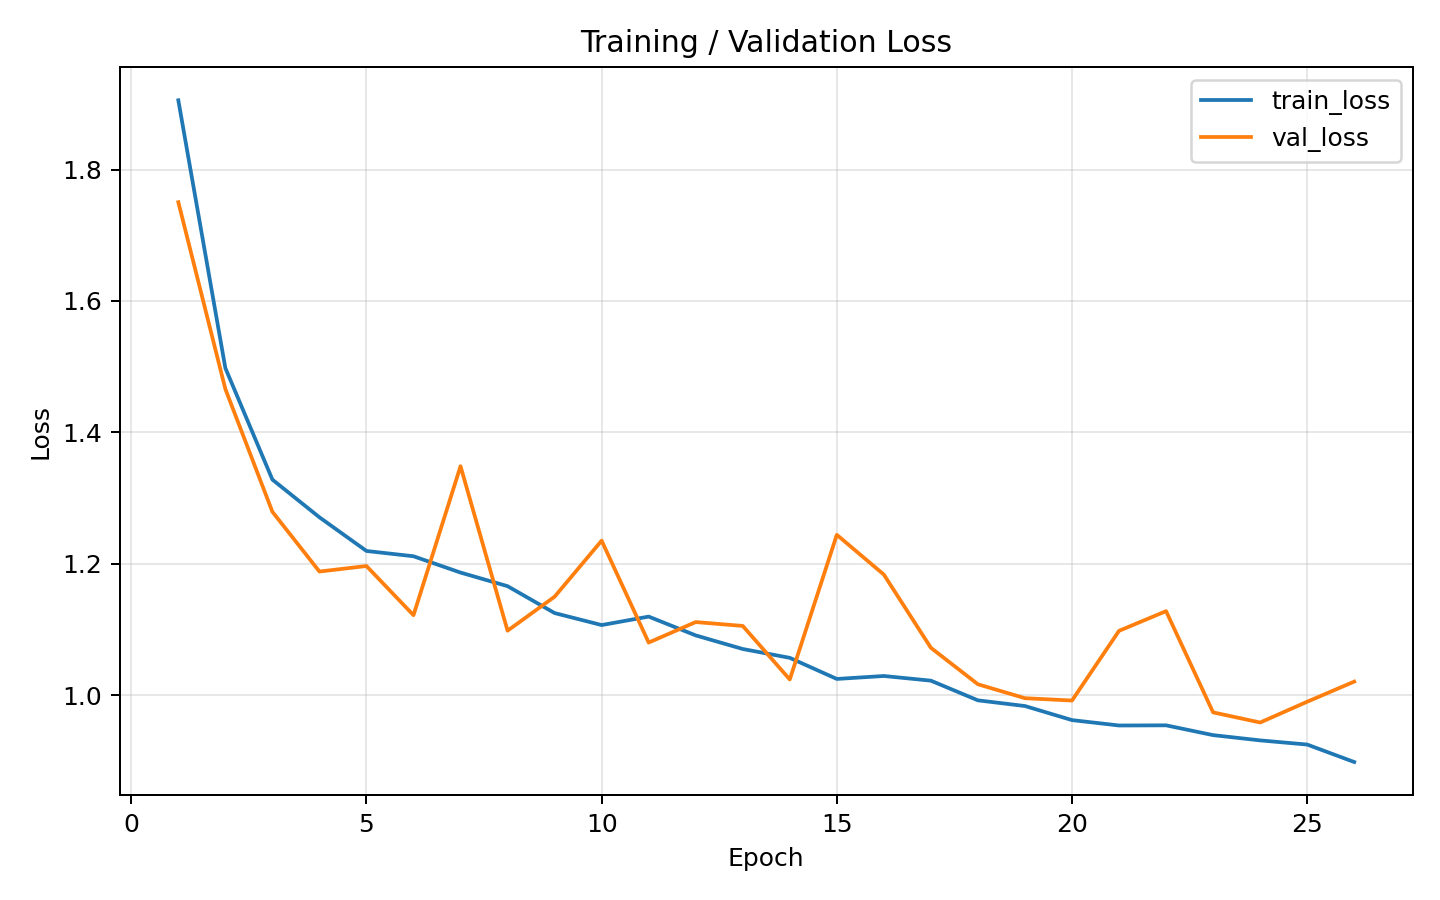
\includegraphics[width=0.86\textwidth]{figures/loss_curve.png}
\caption{训练集与验证集 Loss 曲线}
\label{fig:loss}
\end{figure}

图 \ref{fig:accuracy} 展示了训练和验证 accuracy 曲线。训练准确率持续上升，验证准确率也从初始 45.11\% 提升到最高 67.01\%。不过验证准确率在后期有波动，说明 MLP 对图像空间结构的建模能力有限，进一步提升可能需要更好的特征表示或更细致的超参数搜索。

\begin{figure}[H]
\centering
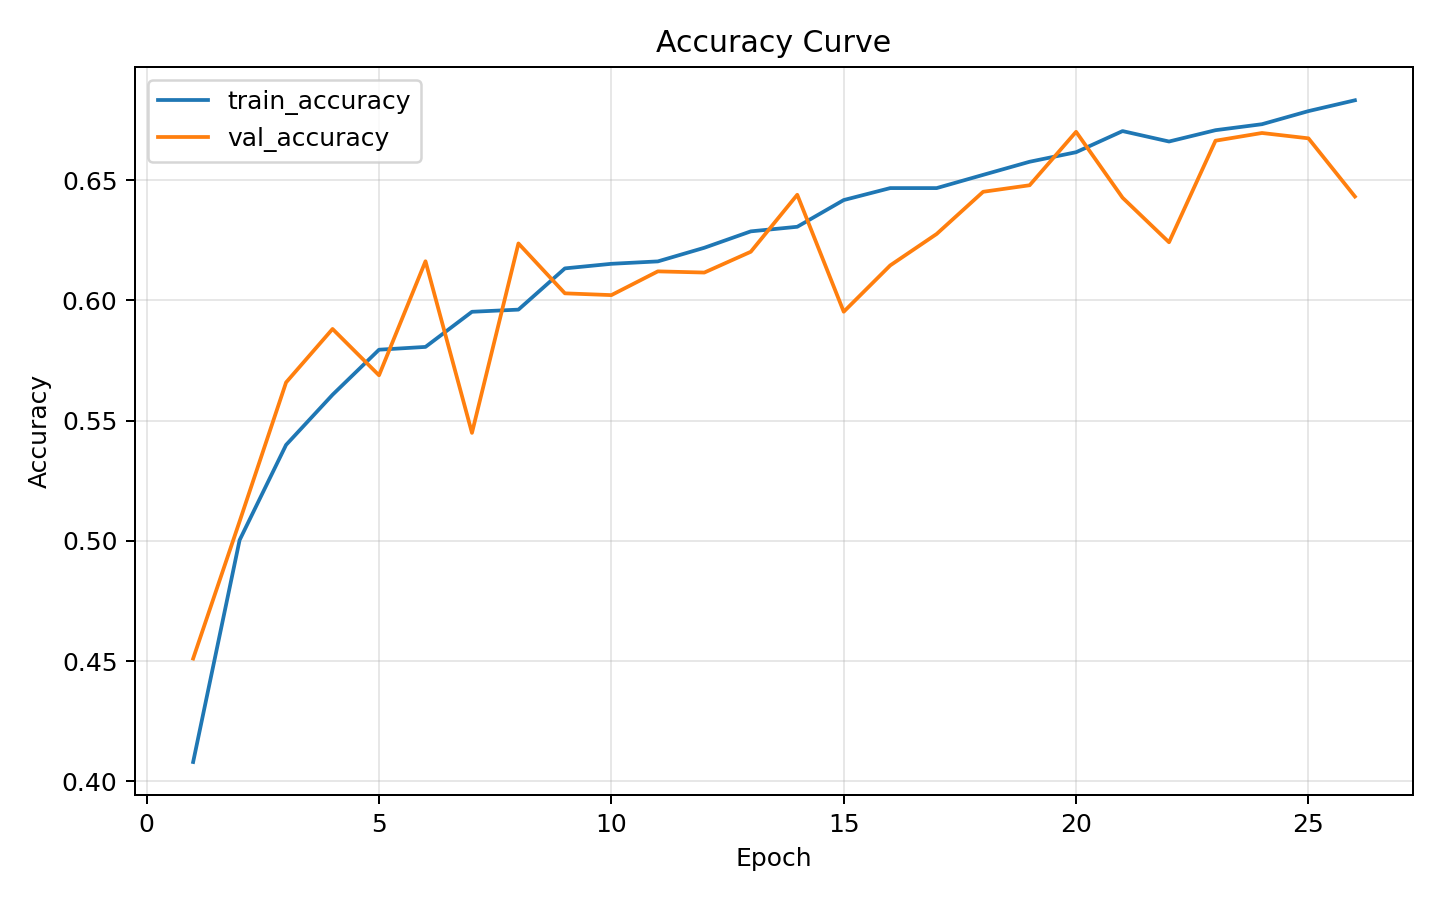
\includegraphics[width=0.86\textwidth]{figures/accuracy_curve.png}
\caption{训练集与验证集 Accuracy 曲线}
\label{fig:accuracy}
\end{figure}

\section{超参数搜索结果}

为了满足作业对参数查找的要求，我使用网格搜索比较了不同学习率、隐藏层维度、激活函数和正则化强度的组合。搜索结果中表现最好的是 learning rate 为 0.01、隐藏层维度为 512、激活函数为 ReLU、weight decay 为 0 的组合，其最佳验证准确率为 65.43\%。

\begin{table}[H]
\centering
\caption{网格搜索最佳结果}
\label{tab:search}
\begin{tabular}{lr}
\toprule
项目 & 取值 \\
\midrule
Trial Index & 21 \\
Learning Rate & 0.01 \\
Hidden Dims & [512] \\
Activation & ReLU \\
Weight Decay & 0 \\
Best Epoch & 19 \\
Best Val Accuracy & 65.43\% \\
\bottomrule
\end{tabular}
\end{table}

从搜索结果可以看出，较大的学习率并不适合该任务，容易导致训练不稳定；ReLU 激活函数整体优于 Sigmoid/Tanh；隐藏层维度为 512 时通常比 256 有更好的表达能力。最终训练配置在搜索结果基础上保留 512 维隐藏层和 ReLU，并加入 weight decay、dropout、数据增强和更长训练，最终取得 67.01\% 的验证准确率。

\section{测试集结果}

训练完成后，我使用验证集表现最好的 checkpoint 在独立测试集上评估。测试集共有 4050 张图像。最终测试准确率为 66.67\%，测试 loss 为 0.9516。

\begin{table}[H]
\centering
\caption{测试集总体结果}
\label{tab:test}
\begin{tabular}{lr}
\toprule
指标 & 数值 \\
\midrule
Test Loss & 0.9516 \\
Test Accuracy & 66.67\% \\
Test Samples & 4050 \\
\bottomrule
\end{tabular}
\end{table}

各类别测试准确率如表 \ref{tab:classacc} 所示。Industrial、Pasture、Forest 和 Residential 准确率较高，而 Highway、River、PermanentCrop 和 AnnualCrop 相对较难分类。

\begin{table}[H]
\centering
\caption{各类别测试准确率}
\label{tab:classacc}
\begin{tabular}{lr}
\toprule
类别 & Accuracy \\
\midrule
AnnualCrop & 55.33\% \\
Forest & 81.56\% \\
HerbaceousVegetation & 68.44\% \\
Highway & 35.47\% \\
Industrial & 85.60\% \\
Pasture & 82.67\% \\
PermanentCrop & 52.80\% \\
Residential & 78.22\% \\
River & 53.60\% \\
SeaLake & 71.78\% \\
\bottomrule
\end{tabular}
\end{table}

图 \ref{fig:cm} 是测试集混淆矩阵。从矩阵可以更直观看出各类别之间的混淆关系。例如 Highway 的识别效果较弱，容易被分到 River、HerbaceousVegetation 或 Residential；PermanentCrop 与 AnnualCrop、HerbaceousVegetation 之间也有较多混淆。这些类别在颜色和纹理上确实比较相似，尤其在 $64 \times 64$ 的低分辨率图像中，线状结构和植被纹理的差异不一定明显。

\begin{figure}[H]
\centering
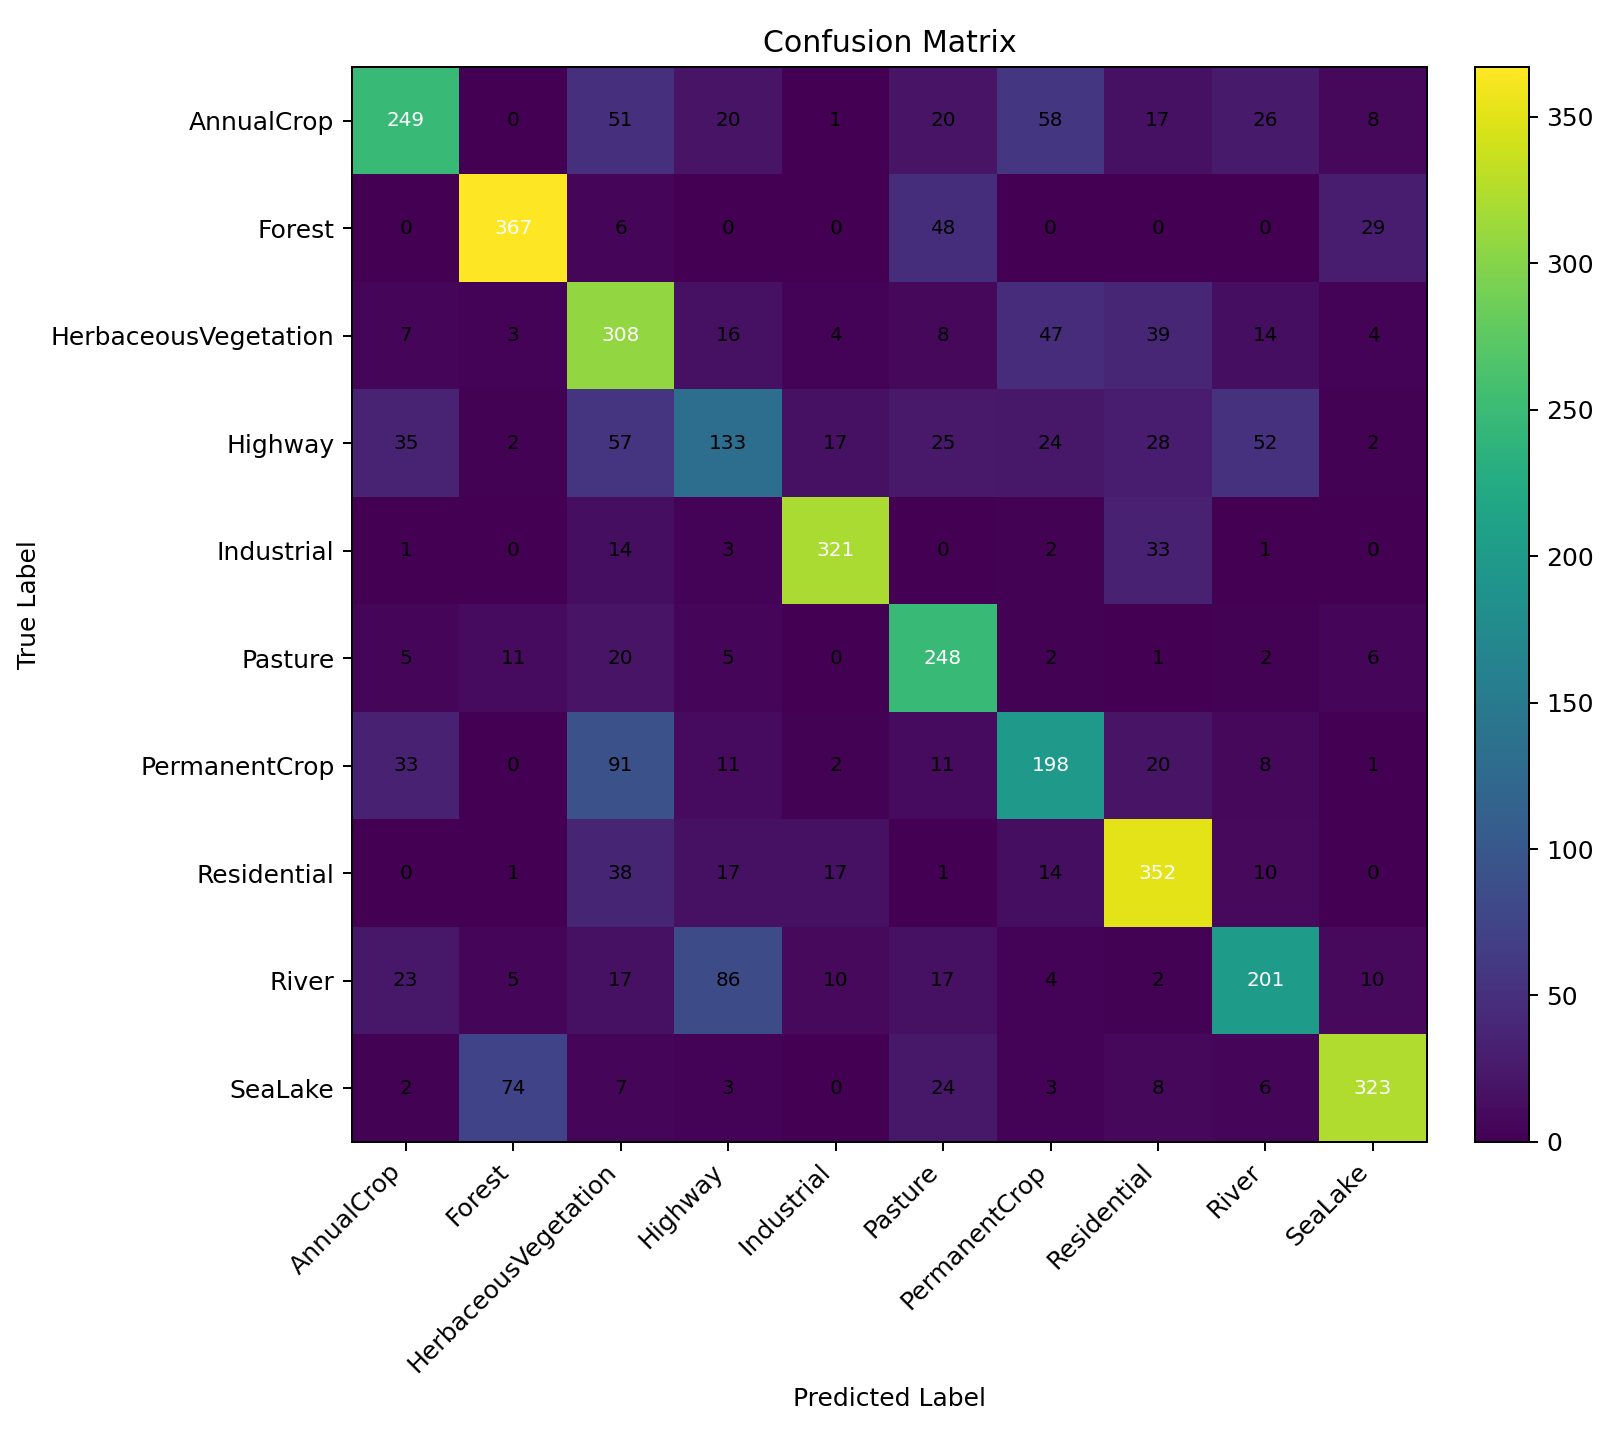
\includegraphics[width=0.92\textwidth]{figures/confusion_matrix.png}
\caption{测试集混淆矩阵}
\label{fig:cm}
\end{figure}

\section{第一层权重可视化}

作业要求将第一层隐藏层权重矩阵恢复成图像尺寸进行观察。由于输入是一张展平后的 RGB 图像，因此第一层中每个隐藏单元都对应一个 $64 \times 64 \times 3$ 的权重图。将这些权重重新 reshape 成图像形式后，可以粗略观察模型第一层关注的颜色和空间模式。

\begin{figure}[H]
\centering
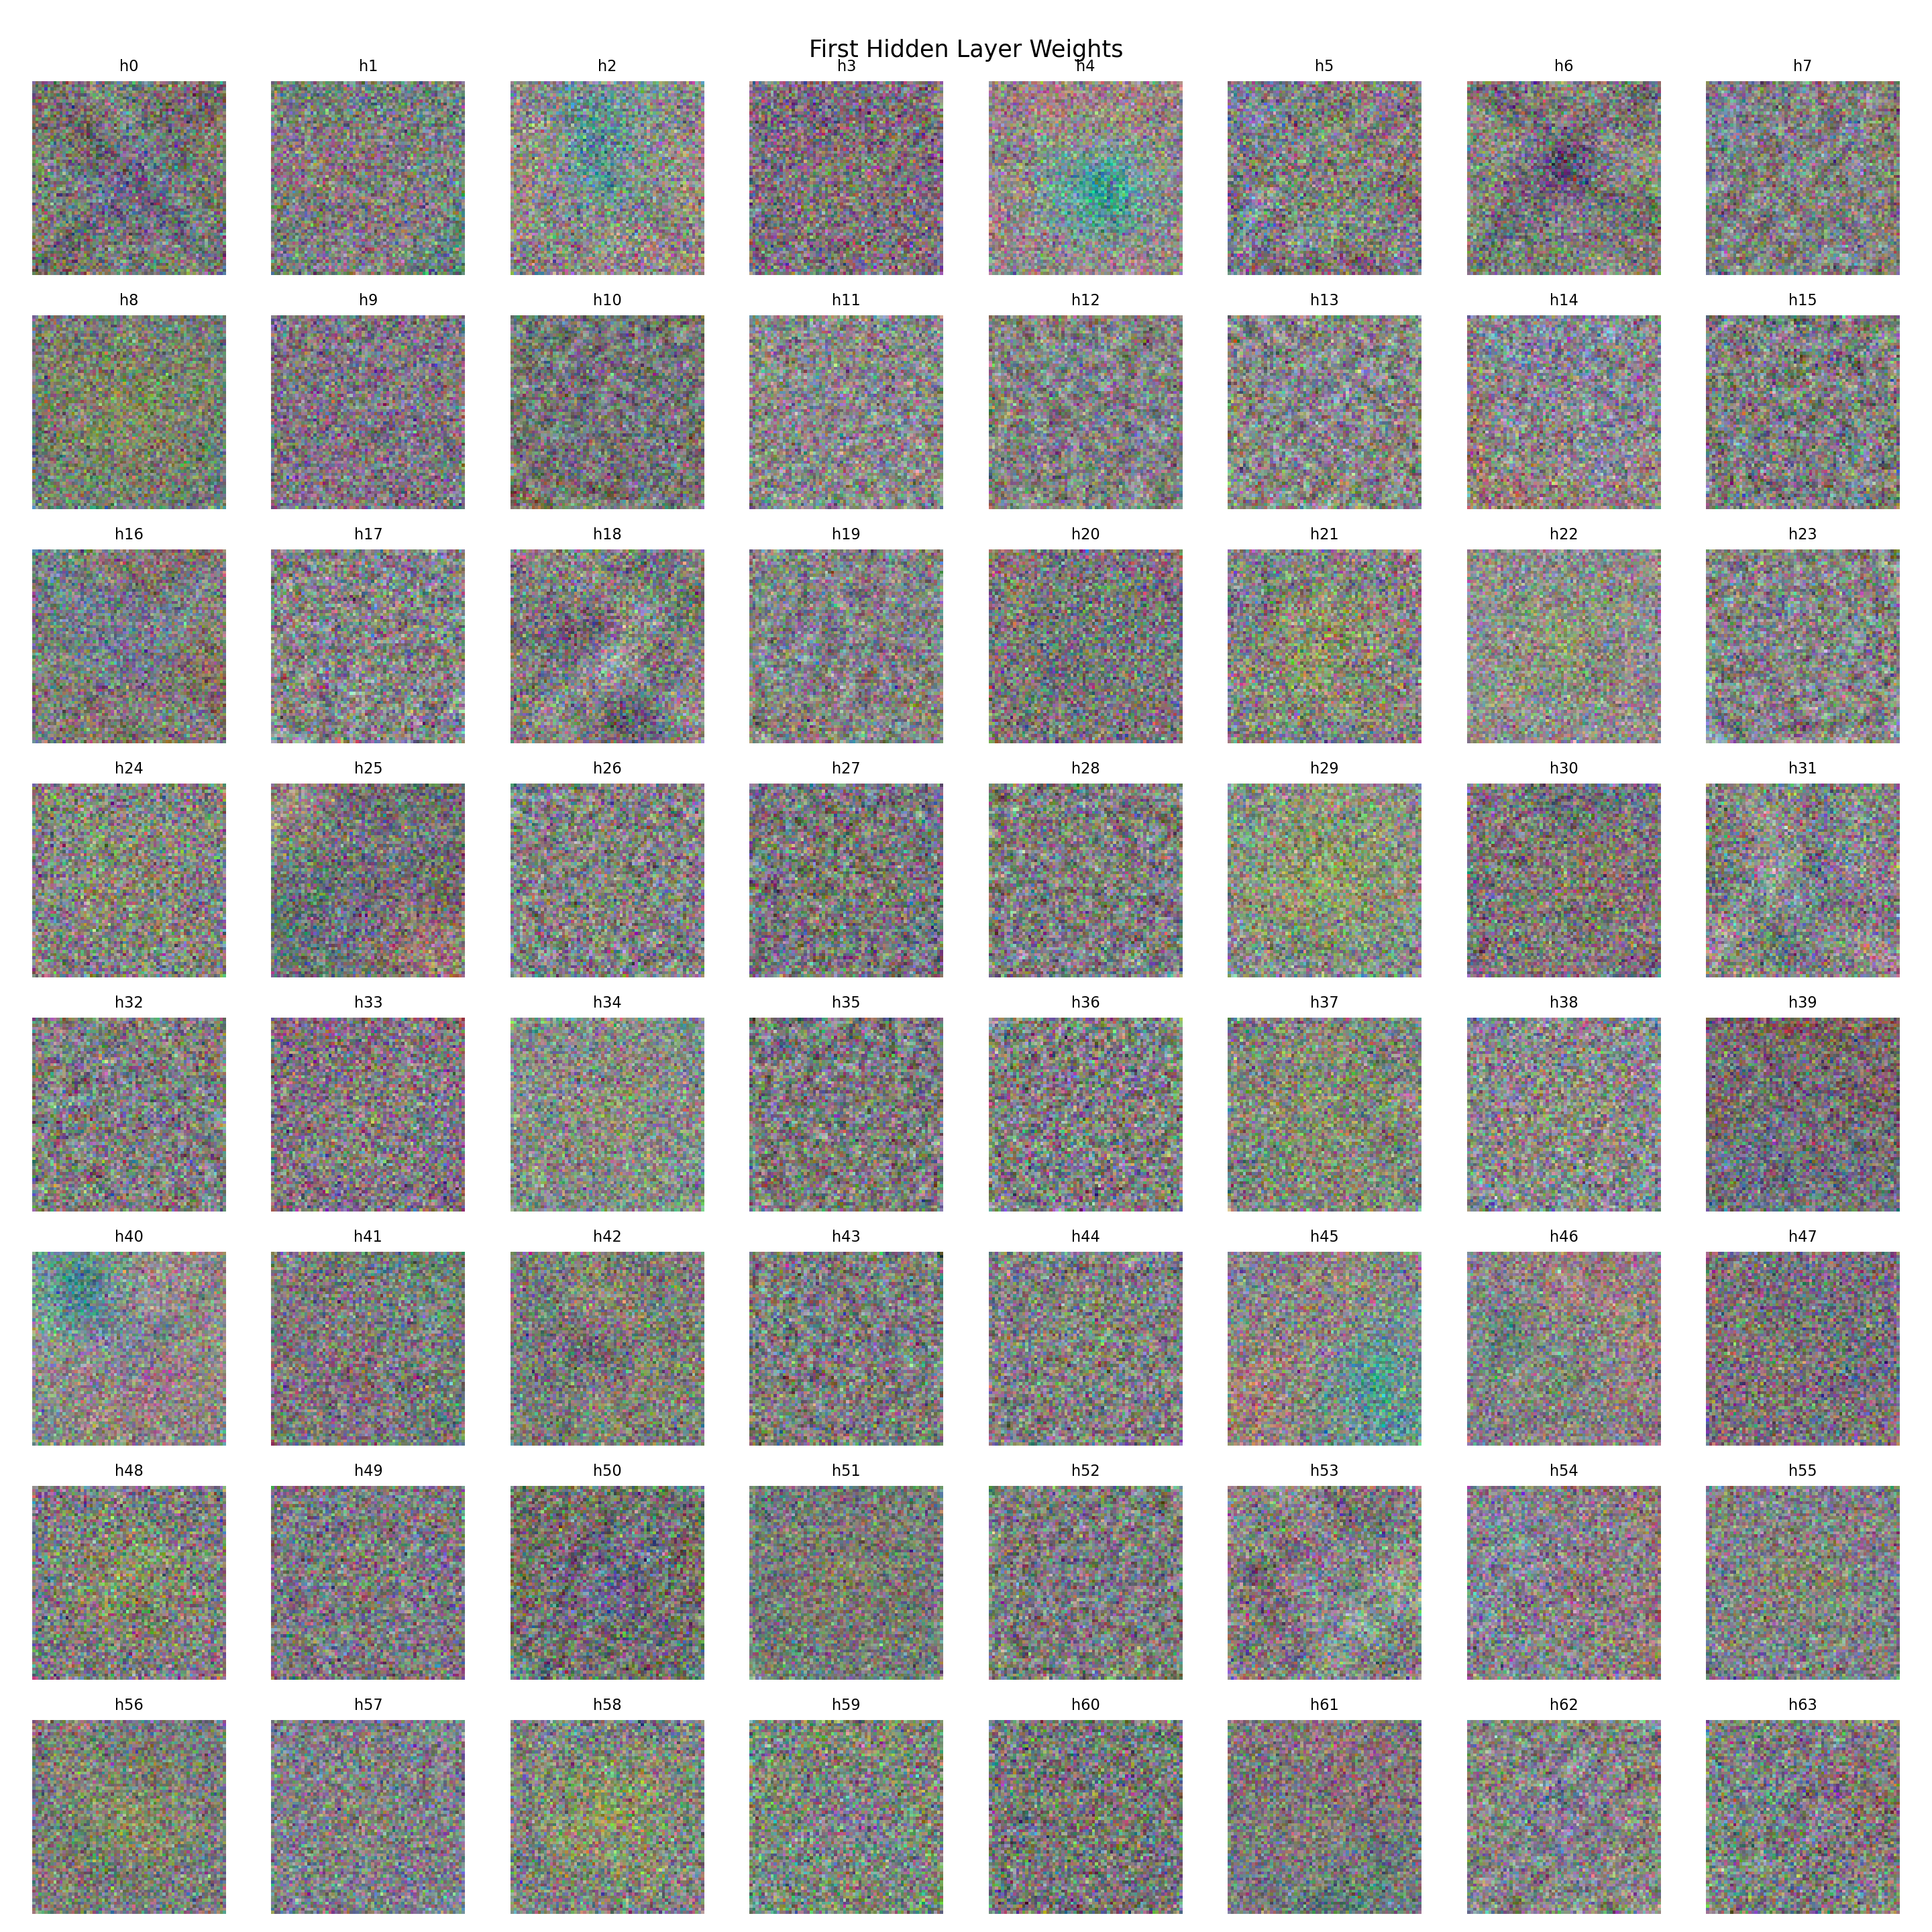
\includegraphics[width=0.9\textwidth]{figures/first_layer_weights.png}
\caption{第一层隐藏层权重可视化}
\label{fig:weights}
\end{figure}

从图 \ref{fig:weights} 可以看到，不同隐藏单元的权重图存在一定差异，有些单元对绿色或蓝色通道更敏感，这可能对应植被、水体等类别中常见的颜色模式。但总体上，这些权重图不像 CNN 卷积核那样具有非常清晰的局部边缘或纹理结构。原因是 MLP 在输入阶段直接把图像展平成一维向量，模型并不知道相邻像素之间的二维空间关系。因此，第一层权重更多体现的是全局颜色分布和粗粒度空间偏好，而不是稳定的局部纹理检测器。

\section{错例分析}

图 \ref{fig:errors} 展示了测试集中若干错分样本。错分样本主要集中在视觉上比较相近的类别之间。

\begin{figure}[H]
\centering
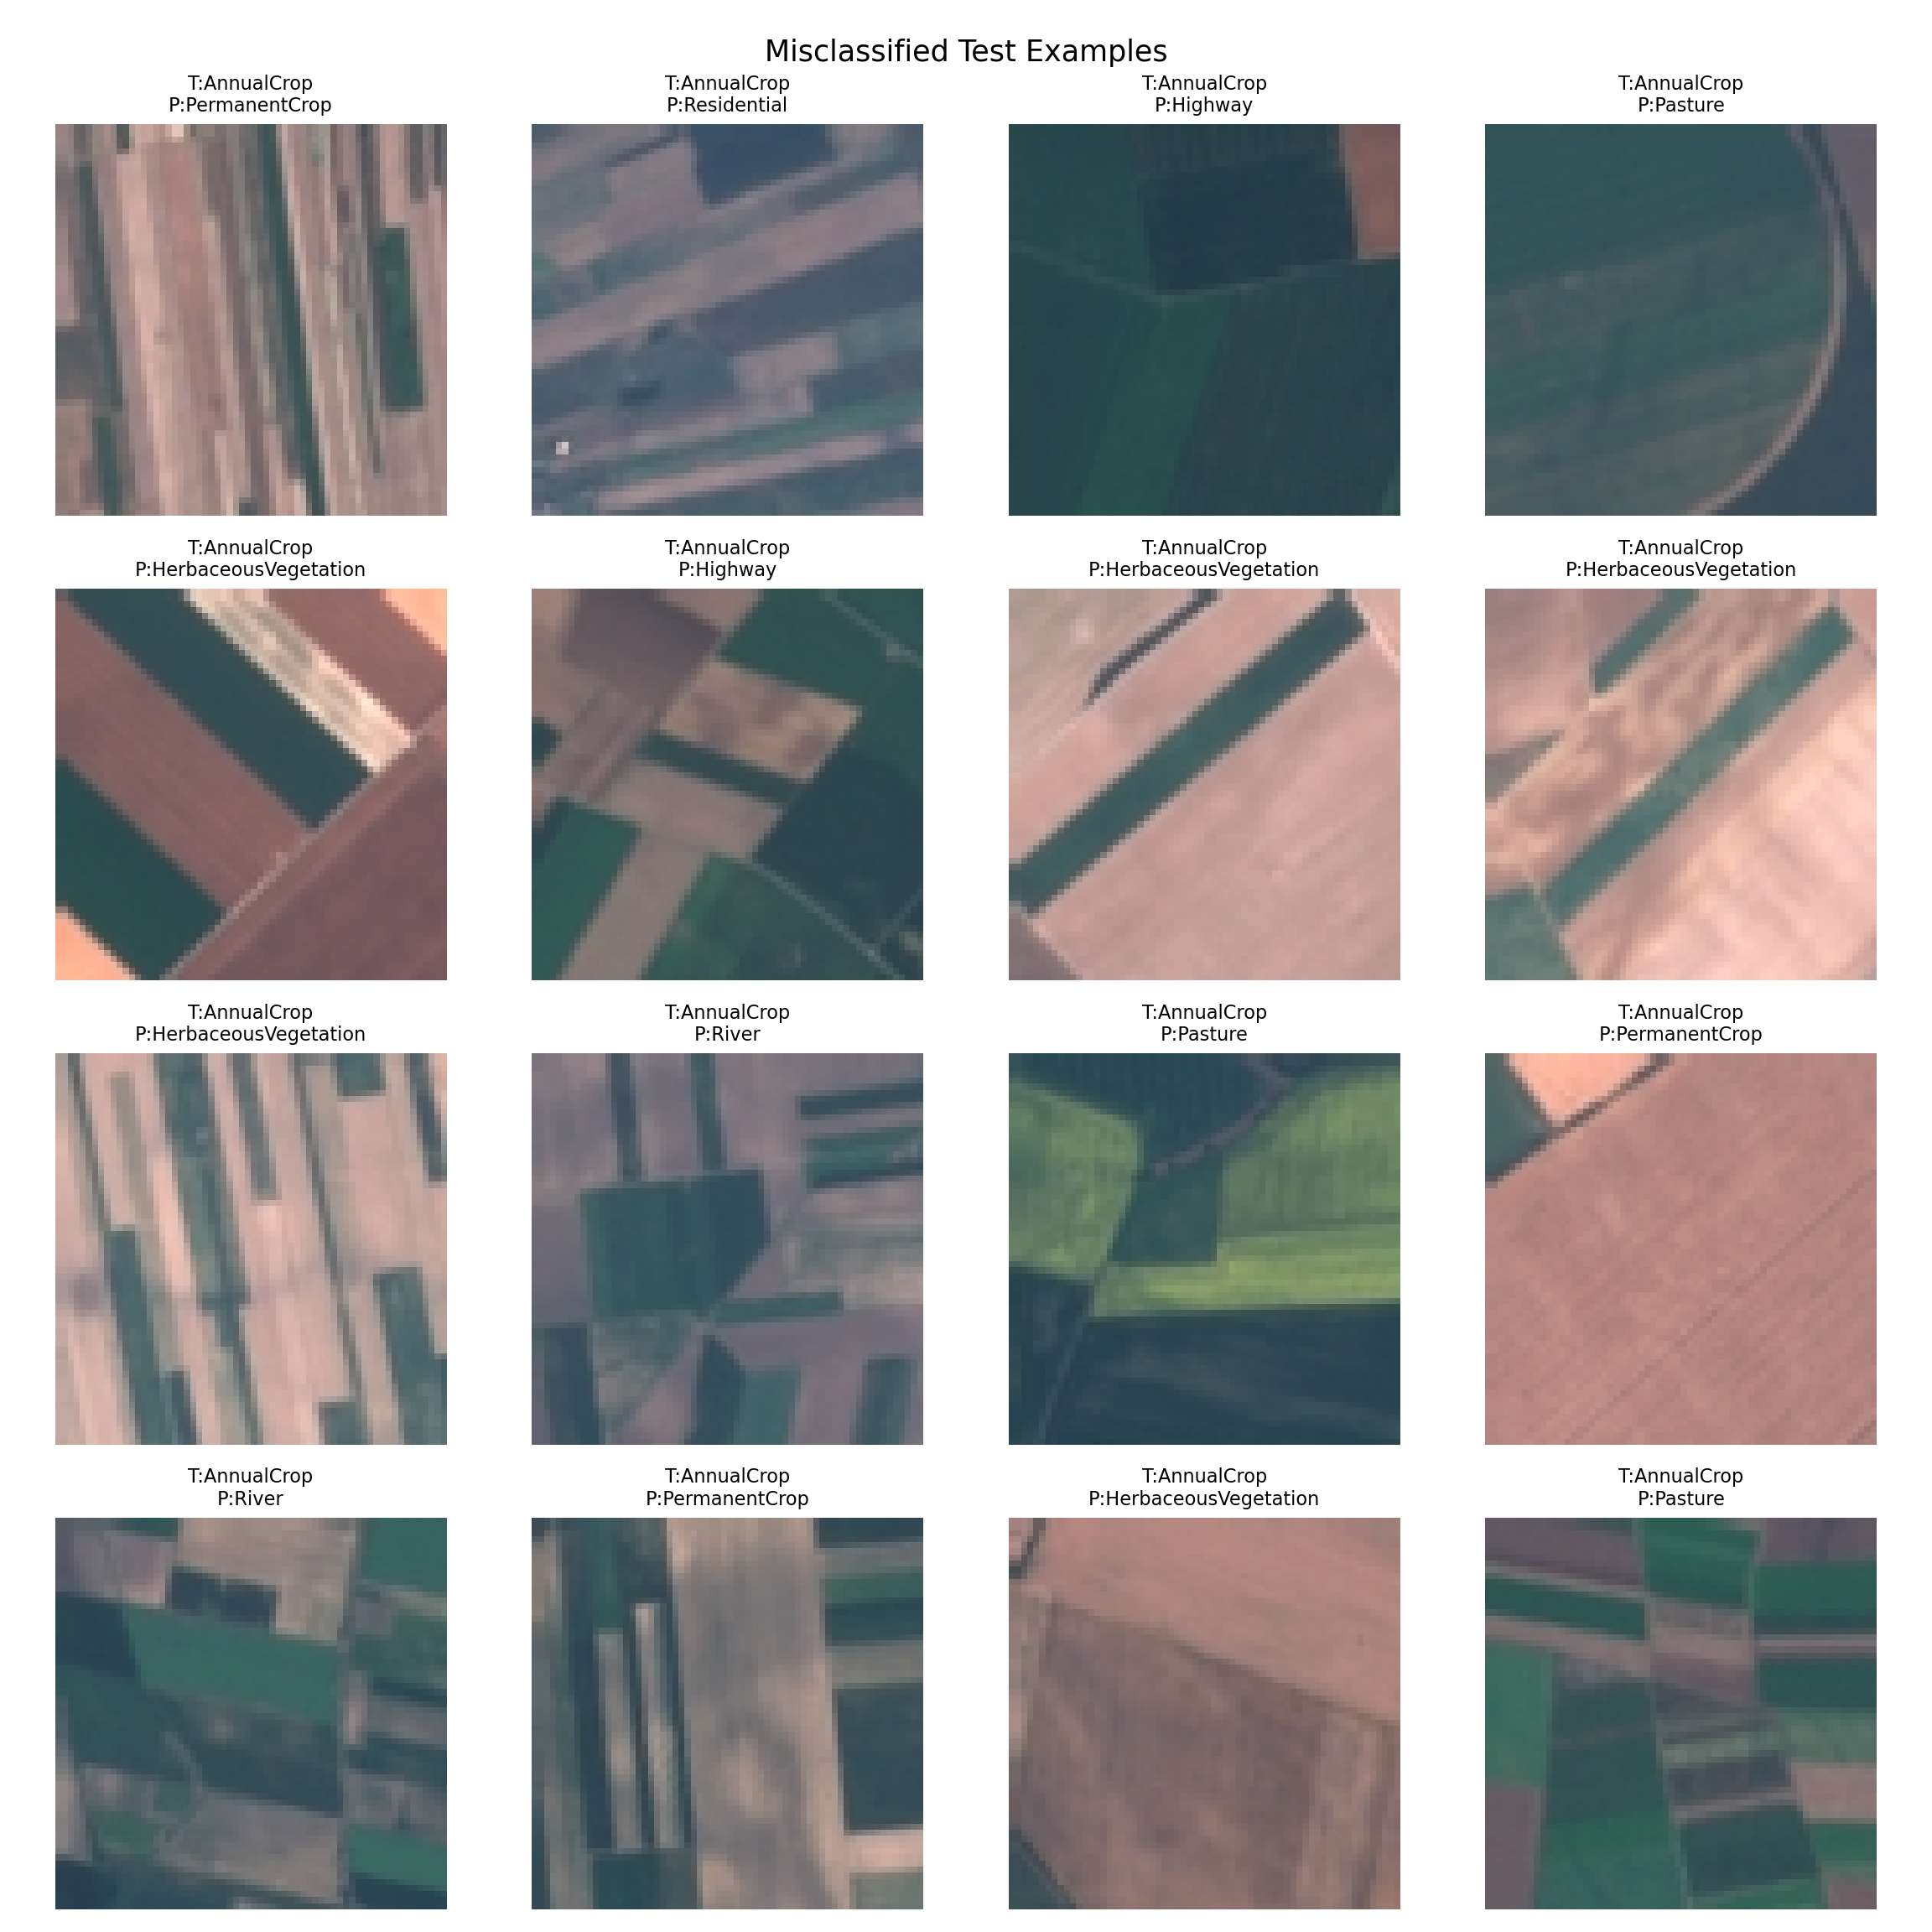
\includegraphics[width=0.88\textwidth]{figures/misclassified_examples.png}
\caption{测试集错例可视化}
\label{fig:errors}
\end{figure}

结合错例图和混淆矩阵，我认为错误主要来自以下几个方面：

\begin{itemize}
    \item Highway 与 River 都可能呈现细长结构，在低分辨率图像中道路和河流的形状特征容易混淆；
    \item AnnualCrop、PermanentCrop 和 HerbaceousVegetation 都包含大量绿色或黄绿色区域，仅靠颜色和全局纹理很难完全区分；
    \item Residential 与 Industrial 有时都包含规则的人造建筑纹理，因此边界不明显；
    \item MLP 缺少卷积结构，不能很好利用局部邻域和空间平移不变性，这是图像分类任务中的明显短板。
\end{itemize}

这些现象说明，MLP 虽然能学习到一定的颜色和整体纹理信息，但对于遥感图像中需要空间结构判断的类别，能力仍然有限。

\section{总结}

本次作业中，我完成了一个从零实现的 EuroSAT MLP 分类器。代码中实现了自动微分、反向传播、MLP 模型、交叉熵损失、L2 正则化、SGD 优化器、学习率衰减、最佳权重保存、超参数搜索、测试评估、混淆矩阵绘制、第一层权重可视化和错例分析。实验结果显示，最终模型在独立测试集上取得 66.67\% 准确率。

通过本次实验，我对神经网络训练流程有了更具体的理解。以前使用深度学习框架时，反向传播和参数更新通常是直接调用接口完成；这次手动实现后，我更清楚地看到每个算子如何保存计算图、如何根据链式法则传播梯度，以及优化器如何根据梯度更新参数。实验也说明，MLP 可以完成基本图像分类，但由于缺少卷积结构，对遥感图像中的局部空间模式利用不足，因此性能存在明显上限。

\section{代码与模型链接}

\begin{itemize}
    \item GitHub Repo：\texttt{TODO: add GitHub link}
    \item 模型权重下载链接：\texttt{TODO: add model weight link}
\end{itemize}

\end{document}
